\documentclass[letterpaper, oneside]{book}
%\usepackage{lingmacros}
\usepackage{tree-dvips}
\usepackage{amsmath}
\usepackage{listings}
\usepackage{graphicx}
\usepackage{xcolor}
\usepackage{mdframed}
\usepackage{fancyhdr}
\usepackage[export]{adjustbox}
\usepackage[skip=10pt]{parskip}
\usepackage{amsfonts}
\usepackage{hyperref}
\usepackage{algorithm}
\usepackage{algpseudocode}
\usepackage{amsthm}
\usepackage{amssymb}
\usepackage{enumerate}
\pagestyle{plain}
\theoremstyle{definition}
\newtheorem{definition}{Definition}[chapter]
\theoremstyle{remark}
\newtheorem*{remark}{Remark}
\newtheorem{theorem}{Theorem}[chapter]
\newtheorem{corollary}{Corollary}[theorem]
\newtheorem{lemma}[theorem]{Lemma}
\newtheorem{prop}{Proposition}[chapter]

% No spaceing between items in itemize
\usepackage{enumitem}
\setlist[itemize]{noitemsep}

% Configure listings backage for code
\lstset{
	%numbers=left,
	%numberstyle=\tiny,
	breaklines=true,
	%numbersep=5pt,
    frame = single,
    aboveskip=2\baselineskip,
    belowskip=2\baselineskip,
	xleftmargin=.15in,
	xrightmargin=.05in}


\lstdefinestyle{python}{
	language=Python,
	basicstyle=\ttfamily\small,
	keywordstyle=\color{blue}\bfseries,
	stringstyle=\color{red},
	commentstyle=\color{gray},
	morekeywords={self}, % Add keywords here
	numbers=left,
	numberstyle=\tiny\color{gray},
	stepnumber=1,
	numbersep=10pt,
	showstringspaces=false,
	breaklines=true,
	frame=lines,
}

\lstdefinestyle{rust}{
	language=Rust,
	basicstyle=\ttfamily\small,
	keywordstyle=\color{blue}\bfseries,
	stringstyle=\color{red},
	commentstyle=\color{gray},
	morekeywords={self}, % Add keywords here
	numbers=left,
	numberstyle=\tiny\color{gray},
	stepnumber=1,
	numbersep=10pt,
	showstringspaces=false,
	breaklines=true,
	frame=lines,
	framextopmargin=1pt
}

\lstdefinestyle{bash}{
	language=Bash,
	basicstyle=\ttfamily\small,
	keywordstyle=\color{blue}\bfseries,
	stringstyle=\color{red},
	commentstyle=\color{gray},
	morekeywords={}, % Add keywords here
	numbers=left,
	numberstyle=\tiny\color{gray},
	stepnumber=1,
	numbersep=10pt,
	showstringspaces=false,
	breaklines=true,
	frame=lines,
	framextopmargin=1pt
}


\graphicspath{{./images/}}

\newenvironment{question}
{\textbf{Question.} }{}


\begin{document}

\tableofcontents


\chapter{Introduction}

\begin{itemize}
	\item Kubernetes abstracts away the hardware infrastructure and exposes your whole data-center as a single enormous computational resources.
	\item To reduce the number of problems that only show up in production, it would be ideal if applications could run in the exact same environment during development and in production so they have the exact same operating system, libraries, system configuration, networking environment, and everything else.
	\item Ideally, you want the developers to deploy applications themselves without knowing anything about the hardware infrastructure and without dealing with the ops team.
	\item container technologies
	\item When using containers, you can (and should) have one container for each application.
	\item Linux Namespaces
	\item Linux Control Groups (cgroups)
	\item Kubernetes enables you to run your software applications on thousands of computer nodes as if all those nodes were a single, enormous computer.
	\item Kubernetes will expose all of them at a single static IP address and expose that address to all applications running in the cluster. This is done through environment variables.
	\item The IP address of the service stays constant, so clients can always connect to its containers, even when they're moved around the cluster.
	\item On any node where Kubernetes is deployed, Kubernetes can run the app immediately without any help from the sysadmins.
\end{itemize}


\section{Principles}

One of the most fundamental Kubernetes principles. Instead of telling Kubernetes exactly what actions it should perform, you're only declaratively changing the desired state of the system and letting Kubernetes examine the current actual state and reconcile it with the desired state. This is true across all of Kubernetes.

\section{Features}
\begin{itemize}
	\item service discovery
	\item auto scaling
	\item load balancing
	\item self-healing
	\item leader election
\end{itemize}

\section{Concepts}

\begin{itemize}
	\item master node
	\item Kubernetes Control Planes
	\item worker node
	\item ReplicationController: Generally, ReplicationControllers are used to replicate pods (that is, create multiple copies of a pod) and keep them running.
\end{itemize}


\section{Tools}
\begin{itemize}
	\item Minikube
	\item kops
\end{itemize}

\section{Kubernetes Cluster Architecture}

\begin{itemize}
	\item Each node runs Docker, the Kubelet and the kube-proxy. You'll interact with the cluster through the \textit{kubectl} command line client, which issues REST requests to the Kubernetes API server running on the master node.
\end{itemize}


\begin{question}
Where do we run the kubctl command?
\end{question}


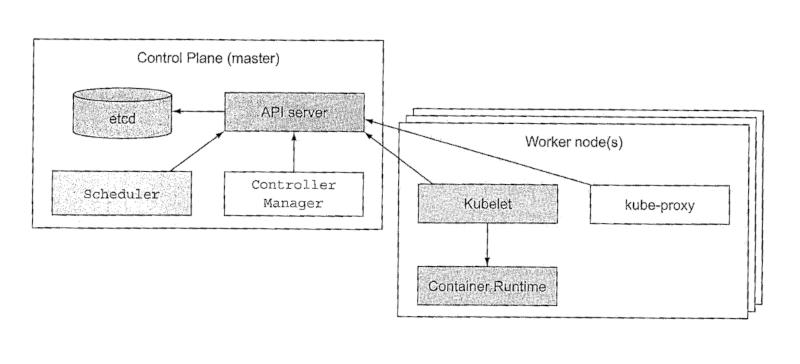
\includegraphics[max width=\textwidth]{introduction/k8s_cluster_architecture.png}

\section{Examples of Commonly Used Commands}

\begin{lstlisting}[style=bash]
kubectl run <ControllerName> --iamge=<ImageName> --port=8080 --generator=run/v1
kubectl expose rc <ControllerName> --type=LoadBalancer --name <ServiceName>
kubectl api-resources
kubectl get pods -o wide
kubectl describe pod <PodName>
\end{lstlisting}

test


\chapter{Docker and Kubernetes}
\chapter{Pod}


A pod is a group of one or more tightly related containers that will always run together on the same worker node and in the same Linux namespace(s). Each pod is like a separate logical machine with its own IP, hostname, processes, and so on, running a single \emph{application}. The application can be a single process, running in a single container, or it can be a main application process and additional supporting processes, each running in its own container. All the containers in a pod will apear to be running on the same logical machine, whereas containers in other pods, even if they're running on the same worker node, will appear to be running on a different one.

A special service of type LoadBalancer.


The host name of the application is the name of the pod as each pod behaves like a separate independent machine with its own IP address and hostname.

\begin{remark}
	As we can see here that the underlying low-level architecture is completely hidden from developers.
\end{remark}

\begin{itemize}
	\item The basic building block in Kubernetes is the pod.
	\item To make that pod accessbiel from outside the cluster, you need to tell Kubernetes to expose all the pods managed by that ReplicationController as a single Service.
	\item The pod has its own unique private IP address and hostname.
	\item A key characteristic of pods is that tey are ephemeral. A pod may disappear at any time \textemdash because the node it's running on has failed, because someone deleted the pod, or because the pod was evicted from an otherwise healthey node. When any of those occurs, a missing pod is replaced with a new one by the ReplicationController. This new pod gets a different IP address from the pod it's replacing. This is where services com in \textemdash to solve the problem of ever-changing pod IP addresses, as well as exposing multiple pods at a single constant IP and port pair.
\end{itemize}



\begin{center}
	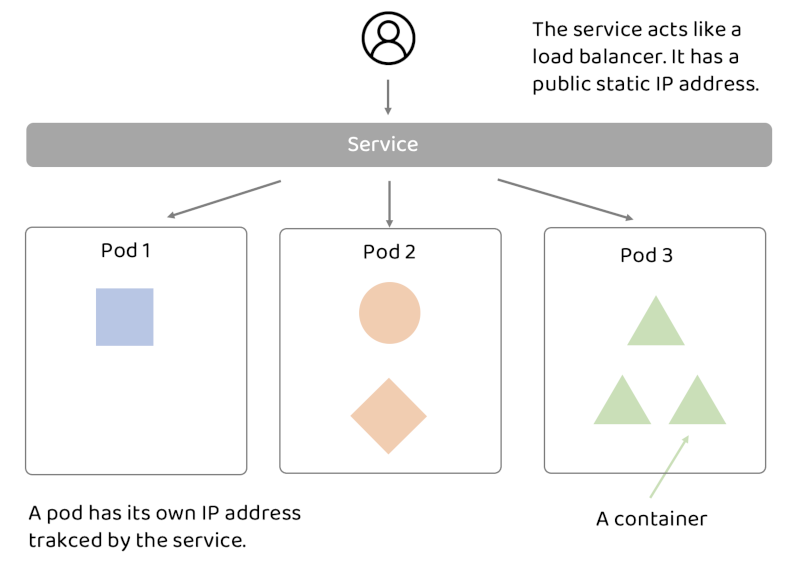
\includegraphics[max width=\textwidth]{pod/k8s_service_and_pod.png}
\end{center}

\chapter{Service}


\begin{itemize}
	\item Services represent a static location for a group of one or more pods that all provde the same service.
\end{itemize}

\end{document}



